\documentclass{article}

\def\ParSkip{} 
\input{../../common/ryantibs}
\usepackage[normalem]{ulem}

\title{Conformal Prediction Under Distribution Shift \\ \smallskip
\large Advanced Topics in Statistical Learning, Spring 2023 \\ \smallskip
Ryan Tibshirani }
\date{}

\begin{document}
\maketitle
\RaggedRight
\vspace{-50pt}

Note: we're following the context, problem setup, notation, etc. from the last
lecture on conformal prediction.

In this lecture we cover conformal (or conformal-like) methods that apply beyond
the i.i.d.\ setting. This is a very active and recent topic of research, and
it's possible (or even likely) that what's considered fundamental in this area  
will change in the next couple of years. Until then, there will be numerous
interesting topics from which we can ``pick and choose'' for a lecture like this
one. We've chosen three such topics (and shamelessly, for two of the topics,
you'll notice an overlap between the authors list and the author of these
lecture notes).  

\section{Likelihood-weighted conformal prediction}

We first cover a likelihood-weighted conformal prediction method, due to
\citet{tibshirani2019conformal}. A primary motivation will be the setting of  
\emph{covariate shift}, where 
\begin{equation}
\label{eq:cov_shift}
\begin{gathered}
(X_i, Y_i) \sim P = P_X \times P_{Y|X}, \; \text{independently, for
  $i=1,\dots,n$} , \\
(X_{n+1}, Y_{n+1}) \sim \widetilde{P} = \widetilde{P}_X \times P_{Y|X}, \;
\text{independently}.
\end{gathered}
\end{equation}
Notice that the conditional distribution of $Y|X$ is assumed to be the same for 
both the training and test data, but the distribution of $X$ is allowed to
change, i.e., we allow \smash{$\widetilde{P}_X \not= P_X$}. This is a general
framework of great interest, because it encompasses may important problem
settings. For example, we could have done some kind of structured covariate
sampling for our training set (demographically, geographically, etc.) but then
we do prediction ``in the wild'', where the mix of covariates is different.

The first thing we could ask is: does this even matter for conformal prediction?
That is, if we observed data according to \eqref{eq:cov_shift}, and computed the 
usual conformal prediction intervals, then would we see a problem with coverage?
The top row of Figure \ref{fig:airfoil} provides an answer, empirically. This is 
taken from \citet{tibshirani2019conformal}, and shows the results of an
experiment in which, over 5000 repetitions, two test sets are drawn: one without  
covariate shift (results in red), and one with covariate shift (in blue). The
top left panel shows the test coverage of split conformal pediction intervals
(drawn as histograms, over the 5000 repetitions). We can see that coverage fails
quite noticeably in the covariate shift setting.

\begin{figure}[htb]
\hspace{-25pt}
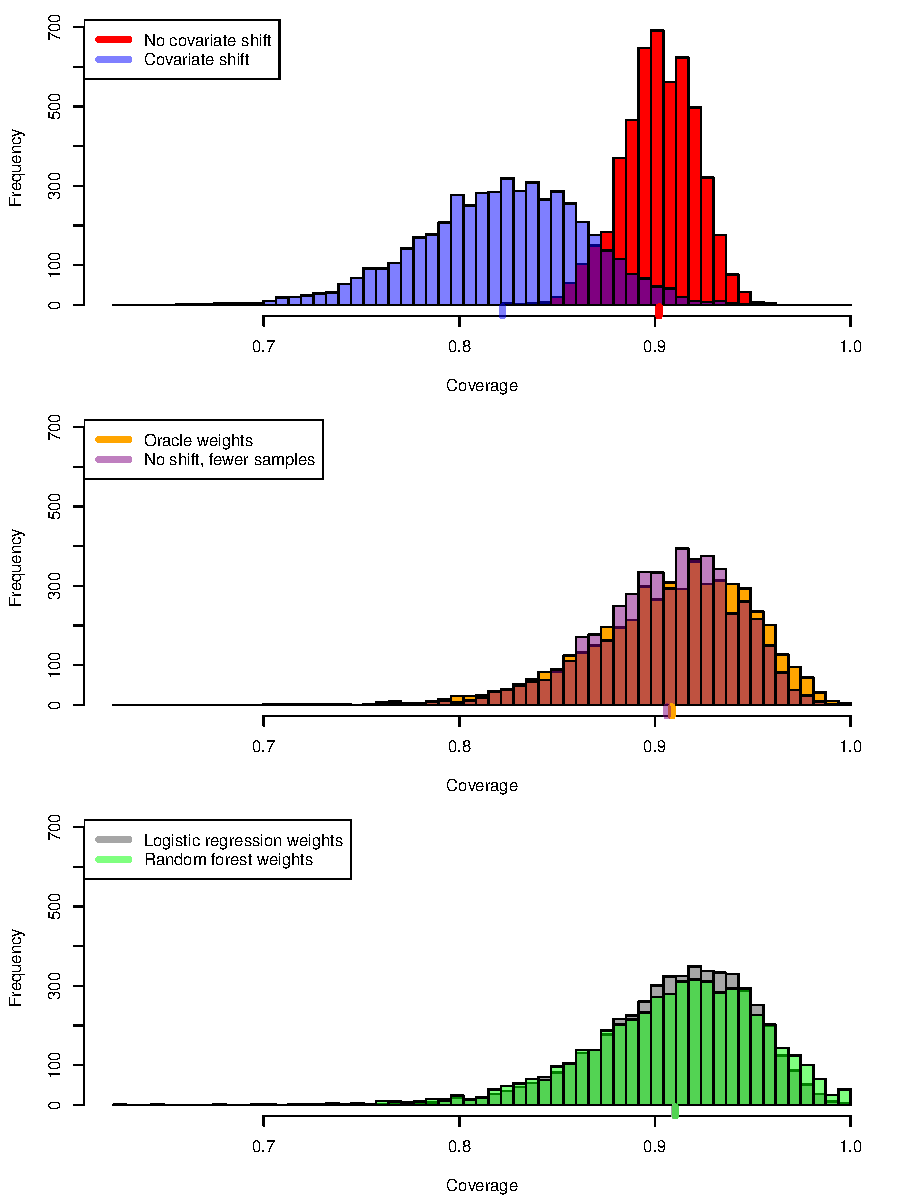
\includegraphics[width=0.525\textwidth]{airfoil_cov.pdf}
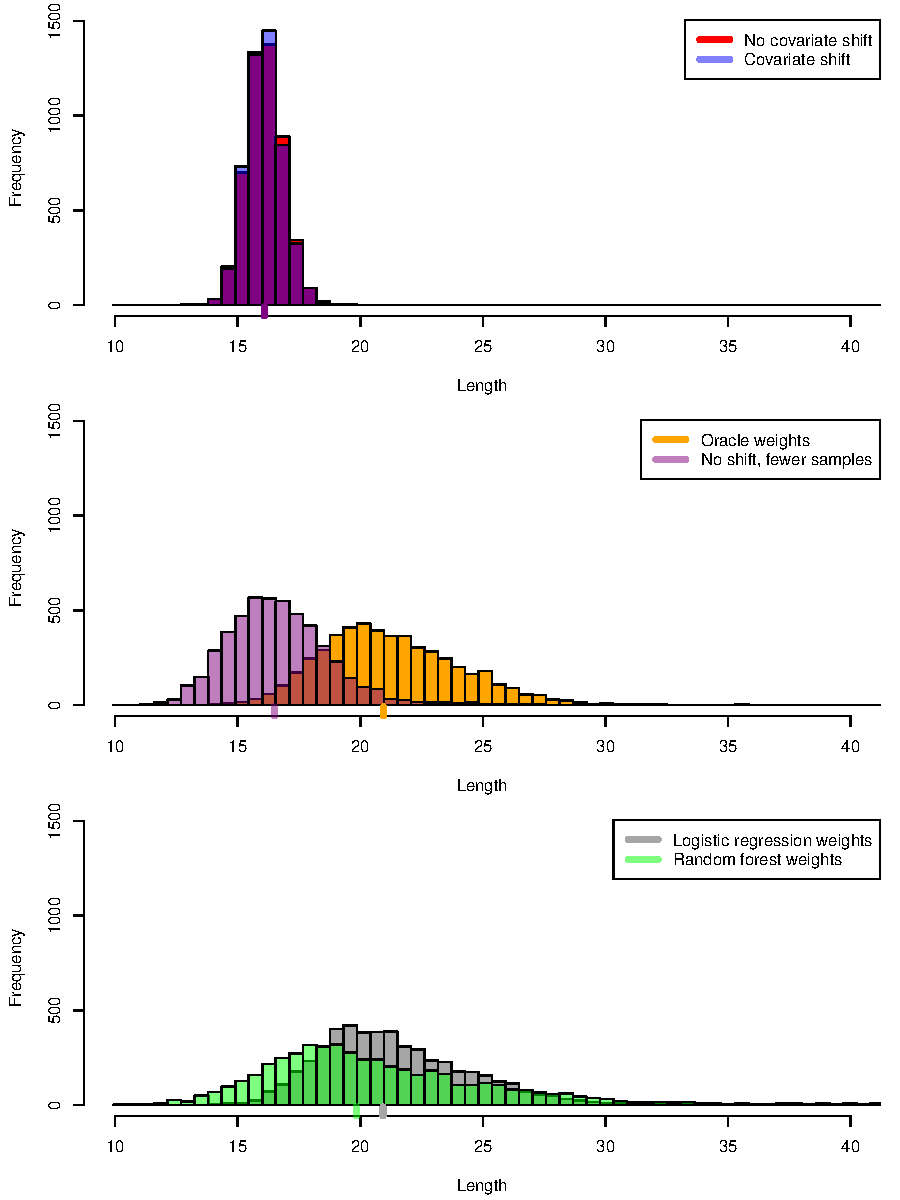
\includegraphics[width=0.525\textwidth]{airfoil_len.pdf}
\caption{\it Experiments for conformal prediction under covariate shift. All
  results are aggregated over 5000 repetitions, each of which randomly forms
  training and test sets. Top row: the usual conformal prediction with and
  without covariate shift. Middle row: weighted conformal prediction using the
  true (and in general unknown) likelihood ratio between test and training
  covariate feature distributions, compare to the usual conformal prediction
  without covariate shift but in a problem with a comparable effective sample 
  size. Bottom row: weighted conformal prediction using an estimated likelihood 
  ratio by running classification with logistic regression or random forests. 
  Credit: \citet{tibshirani2019conformal}.}      
\label{fig:airfoil}
\end{figure}

To remedy this, we are going to work with a weighed empirical distribution of 
conformity scores, rather than the usual (unweighted) empirical distribution. 
And to approach this argument, it helps to build intuition by looking back at
the first key idea behind conformal, which recall, used ranks in order to
construct adjusted empirical quantiles. 

\paragraph{Revisiting the first key idea: rank-based quantiles.}

\def\Quantile{\mathrm{Quantile}}

The last lecture proved the following fact. If $R_1,\dots,R_{n+1}$ are
exchangeable random variables, then for any $\alpha \in (0,1)$, 
\[
\P\bigg\{ R_{n+1} \leq \Quantile\bigg( \frac{\lceil (1-\alpha)(n+1) \rceil}{n};
\, \frac{1}{n} \sum_{i=1}^n \delta_{R_i} \bigg) \bigg\} \geq 1-\alpha.
\]
We can equivalently express this as
\[
\P\bigg\{ R_{n+1} \leq \Quantile\bigg( \frac{\lceil (1-\alpha)(n+1) \rceil}{n+1}; 
\, \frac{1}{n+1} \sum_{i=1}^{n+1} \delta_{R_i} \bigg) \geq 1-\alpha,
\]
because the event in each of the last two displays is equivalent to the
statement that $R_{n+1}$ is among the \smash{$\lceil (1-\alpha)(n+1) \rceil$}
smallest of $R_1,\dots,R_{n+1}$. The last display is itself equivalent to
\[
\P\bigg\{ R_{n+1} \leq \Quantile\bigg( 1-\alpha; \, \frac{1}{n+1}
\sum_{i=1}^{n+1} \delta_{R_i} \bigg) \bigg\} \geq 1-\alpha, 
\]
because the quantile function of the empirical distribution of
$R_1,\dots,R_{n+1}$, only changes in increments of $1/(n+1)$ (and will
automatically round up to the nearest increment until it captured sufficient
probability mass to exceed $1-\alpha$). Finally, it turns out that we can
equivalently express the last display as  
\begin{equation}
\label{eq:quantile}
\P\bigg\{ R_{n+1} \leq \Quantile\bigg( 1-\alpha; \, \frac{1}{n+1} \sum_{i=1}^n
\delta_{R_i} + \frac{1}{n+1} \delta_\infty \bigg) \bigg\} \geq 1-\alpha.
\end{equation}
This can be seen by applying the following fact to the complements of the two
events in the previous two displays: for a discrete distribution $F$ with
support points $a_1,\dots,a_k \in \R$, denoting $q=\Quantile(\beta; F)$, if we
reassign the points $a_i > q$ to arbitrary values strictly larger than $q$,
yielding a new distribution $F'$, then the level $\beta$ quantile remains
unchanged, $\Quantile(\beta; F) = \Quantile(\beta; F')$.  

\paragraph{Alternate proof of the quantile result \eqref{eq:quantile}.}

We will now prove \eqref{eq:quantile} from a new perspective (no longer by
reducing it to a statement about the rank of $R_{n+1}$ among
$R_1,\dots,R_{n+1}$) that will enable us to extend this result to a more general
setting. The basic idea is to condition on the unlabeled collection of values
obtained by our random variables $R_1,\dots,R_{n+1}$, then inspect the
probabilities that the last random variable $R_{n+1}$ attains each one of these
values.  

Denote by $f$ the probability density function (or mass function, or more
generally, Radon-Nikodym derivative with respect to an arbitrary base measure)
of the joint sample $R_1,\dots,R_{n+1}$. Exchangeability means
\[
f(r_1,\dots,r_{n+1}) = f(r_{\sigma(1)}, \dots, r_{\sigma(n+1)}), \quad \text{for 
  all permutations $\sigma$}.
\] 
For simplicity, and without loss of generality, assume that there are almost
surely no ties among the scores $R_1,\dots,R_{n+1}$. Let $E_r$ be the event that 
$\{R_1,\dots,R_{n+1}\}=\{r_1,\dots,r_{n+1}\}$. Then for each $i$,  
\begin{align*}
\P(R_{n+1}=r_i \,|\, E_r)
&= \frac{\sum_{\sigma : \sigma(n+1)=i} f(r_{\sigma(1)}, \dots, r_{\sigma(n+1)})}  
{\sum_\sigma f(r_{\sigma(1)}, \dots, r_{\sigma(n+1)})} \\
&= \frac{\sum_{\sigma: \sigma(n+1)=i} f(r_1, \dots, r_{n+1})}  
{\sum_\sigma f(r_1, \dots, r_{n+1})} \\
&= \frac{n!}{(n+1)!} = \frac{1}{n+1}. 
\end{align*}
This shows that the distribution of $R_{n+1}|E_r$ is uniform on the set 
$\{r_1,\dots,r_{n+1}\}$, that is,
\[
R_{n+1}|E_r \sim \frac{1}{n+1}\sum_{i=1}^{n+1}\delta_{r_i},
\]
and it follows, since $F(Q(t)) \geq t$ for any cumulative distribution function
$F$ and corresponding quantile function $Q$, that   
\[
\P\bigg\{ R_{n+1} \leq \Quantile\bigg( 1-\alpha; \,
\frac{1}{n+1}\sum_{i=1}^{n+1}\delta_{r_i} \bigg) \, \bigg| \, 
E_r\bigg\} \geq 1-\alpha,
\]
This is the same as
\[
\P\bigg\{ R_{n+1} \leq \Quantile\bigg( 1-\alpha; \,
\frac{1}{n+1}\sum_{i=1}^{n+1}\delta_{R_i}\bigg) \, \bigg| \,  
E_r\bigg\} \geq 1-\alpha,
\]
and we can marginalize to obtain   
\[
\P\bigg\{ R_{n+1} \leq \Quantile\bigg( 1-\alpha; \,
\frac{1}{n+1}\sum_{i=1}^{n+1}\delta_{R_i}\bigg) \bigg\} \geq 1-\alpha.
\]
This is the display right above \eqref{eq:quantile}, and by the same argument as
given above, it is equivalent to \eqref{eq:quantile}.

\subsection{Weighted exchangeability: quantile lemma}

Though the alternate proof we just gave is a bit longer than the standard
reduction to ranks, it is important because it allows us to move past the
setting of exchangeable scores $R_1,\dots,R_{n+1}$. In words, after revealing
(conditioning on) the set of values obtained by the scores, we need to be able
to answer the following question: \emph{what is the probability with which any
  given value is that of the test score?}   

This question still has a relatively clean answer when $R_1,\dots,R_{n+1}$ are
\emph{weighted exchangeable}, which is a generalization of exchangeability, and
specifies that the random variables have a density (or mass function, or more
generally, Radon-Nikodym derivative with respect to an arbitrary base measure)
of the form   
\begin{equation}
\label{eq:weighted_exch}
f(r_1,\dots,r_{n+1}) = \prod_{i=1}^{n+1} w_i(r_i) \cdot g(r_1,\dots,r_{n+1}),  
\end{equation}
where $g$ is any function that is permutation invariant, i.e.,
\smash{$g(r_1,\dots,r_{n+1}) = g(r_{\sigma(1)}, \dots, r_{\sigma(n+1)})$}, for
any permutation $\sigma$.

We now have the following extension of \eqref{eq:quantile}, stated as a lemma,
for concreteness.  

\begin{lemma}
\label{lem:weighted_quant}
Let $Z_i$, $i=1,\dots,n+1$ be weighted exchangeable random variables, with
respect to weight functions $w_1,\dots,w_{n+1}$. Assume without loss of
generality that these are distinct almost surely. Let 
\[
R_i = V\big( Z_i; \, \{Z_1,\dots,Z_{n+1}\} \big), \quad i=1,\dots,n+1, 
\]
where $V$ is an arbitrary score function, and define
\begin{equation}
\label{eq:weighted_prob}
p^w_i(z_1,\dots,z_{n+1}) = 
\frac{\sum_{\sigma : \sigma(n+1)=i} \prod_{j=1}^{n+1} w_j(z_{\sigma(j)})}
{\sum_\sigma \prod_{j=1}^{n+1} w_j(z_{\sigma(j)})}, \quad i=1,\dots,n+1,   
\end{equation} 
where the sums are over permutations $\sigma$ of the numbers $1,\dots,n+1$.
Then for any $\alpha \in (0,1)$,  
\begin{equation}
\label{eq:weighted_quant}
\P\bigg\{ R_{n+1} \leq \Quantile\bigg( 1-\alpha; \, \sum_{i=1}^n 
p^w_i(Z_1,\dots,Z_{n+1}) \delta_{R_i} + p^w_{n+1}(Z_1,\dots,Z_{n+1}) 
\delta_\infty \bigg) \bigg\} \geq 1-\alpha.
\end{equation}
\end{lemma}

\begin{proof}
We follow the same general strategy from the alternate proof of
\eqref{eq:quantile}. Let $E_z$ denote the event that
$\{Z_1,\dots,Z_{n+1}\}=\{z_1,\dots,z_{n+1}\}$, and let $r_i=V(z_i;
\{z_1,\dots,z_{n+1}\})$, for $i=1,\dots,n+1$. Let $f$ be the density function
of the joint sample $Z_1,\dots,Z_{n+1}$. For each $i$, we have
\begin{equation}
\label{eq:general_calc}
\P(R_{n+1} = r_i \,|\, E_z) = \P(Z_{n+1} = z_i \,|\, E_z)
= \frac{\sum_{\sigma : \sigma(n+1)=i} f(z_{\sigma(1)},\dots, z_{\sigma(n+1)})} 
{\sum_\sigma f(z_{\sigma(1)},\dots, z_{\sigma(n+1)})},
\end{equation}
and as $Z_1,\dots,Z_{n+1}$ are weighted exchangeable,
\begin{align*}
\frac{\sum_{\sigma : \sigma(n+1)=i} f(z_{\sigma(1)},\dots, z_{\sigma(n+1)})}  
{\sum_\sigma f(z_{\sigma(1)},\dots, z_{\sigma(n+1)})} &= 
\frac{\sum_{\sigma : \sigma(n+1)=i} \prod_{j=1}^{n+1} w_j(z_{\sigma(j)}) \cdot 
  g(z_{\sigma(1)},\dots,z_{\sigma(n+1)})}
{\sum_\sigma \prod_{j=1}^{n+1} w_j(z_{\sigma(j)}) \cdot
  g(z_{\sigma(1)},\dots,z_{\sigma(n+1)})}  \\
&= \frac{\sum_{\sigma : \sigma(n+1)=i} \prod_{j=1}^{n+1} w_j(z_{\sigma(j)})
  \cdot g(z_1,\dots,z_{n+1})} 
{\sum_\sigma\prod_{j=1}^{n+1} w_j(z_{\sigma(j)}) \cdot g(z_1,\dots,z_{n+1})} \\ 
&= p^w_i(z_1,\dots,z_{n+1}).
\end{align*}
In other words,  
\begin{equation}
\label{eq:weighted_dist}
R_{n+1}|E_z \sim \sum_{i=1}^{n+1} p^w_i(z_1,\dots,z_{n+1})\delta_{r_i},
\end{equation}
which implies that
\[
\P\bigg\{ R_{n+1} \leq \Quantile\bigg( 1-\alpha; \, \sum_{i=1}^{n+1}
p^w_i(z_1,\dots,z_{n+1})\delta_{r_i}\bigg) \, \bigg| \, E_z\bigg\} \geq
1-\alpha.  
\]
This is equivalent to  
\[
\P\bigg\{ R_{n+1} \leq \Quantile\bigg( 1-\alpha; \, \sum_{i=1}^{n+1} 
p^w_i(Z_1,\dots,Z_{n+1}) \delta_{R_i}\bigg) \, \bigg| \, E_z\bigg\} \geq
1-\alpha,  
\]
and after marginalizing, 
\[
\P\bigg\{ R_{n+1} \leq \Quantile\bigg( 1-\alpha; \, \sum_{i=1}^{n+1} 
p^w_i(Z_1,\dots,Z_{n+1}) \delta_{R_i}\bigg) \bigg\} \geq 1-\alpha. 
\]
Finally, by the same arguments as before, we can change the point mass at 
$R_{n+1}$ to one at $\infty$, which proves \eqref{eq:weighted_quant} as
desired. 
\end{proof}

We remark that computation of the probability weights in
\eqref{eq:weighted_prob} is very difficult in general, due to the combinatorial  
form (note that this actually reduces to computing what is known as a
\emph{matrix permanent}, which is known to be hard). However, for cetain
weighted exchangeable structures, it can be easy, as we will see a bit later for
covariate shift. 

\subsection{Weighted exchangeability: conformal prediction}

\def\hC{\hat{C}}

A weighted version of conformal prediction follows from Lemma
\ref{lem:weighted_quant}, which we state next as a theorem, for concreteness. 

\begin{theorem}
\label{thm:weighted_conf}
Assume that $Z_i=(X_i,Y_i) \in \cX \times \cY$, $i=1,\dots,n+1$ are weighted   
exchangeable with weight functions $w_1,\dots,w_{n+1}$. Define a weighted
conformal set (based on the first $n$ samples) at a point $x \in \cX$, with
nominal error level $\alpha \in (0,1)$ as follows. Let   
\begin{equation}
\label{eq:scores}
\begin{aligned}
R_i^{(x,y)} &= V\Big( (X_i,Y_i); \, \{Z_1,\dots,Z_n,(x,y)\} \Big), \quad
  i=1,\dots,n, \\ 
R_{n+1}^{(x,y)} &= V\Big( (x,y); \, \{Z_1,\dots,Z_n,(x,y)\} \Big), 
\end{aligned}
\end{equation}
for an arbitrary score function $V$, and
\begin{equation}
\label{eq:weighted_conf}
\hC_n(x) = \bigg\{ y : R_{n+1}^{(x,y)} \leq \Quantile\bigg( 1-\alpha; 
\, \sum_{i=1}^n p^w_i\big( Z_1,\dots,Z_n,(x,y) \big) \delta_{R_i^{(x,y)}} \,+\, 
p^w_{n+1}\big( Z_1,\dots,Z_n,(x,y) \big) \delta_\infty \bigg) \bigg\},  
\end{equation}
where \smash{$p^w_i$}, $i=1,\dots,n+1$ are as in \eqref{eq:weighted_prob}.  
Then \smash{$\hC_n$} satisfies    
\begin{equation}
\label{eq:weighted_cov}
\P\big( Y_{n+1} \in \hC_n(X_{n+1}) \big) \geq 1-\alpha.  
\end{equation}
\end{theorem}

\begin{proof}
Abbreviate \smash{$R_i=R_i^{(X_{n+1},Y_{n+1})}$}, $i=1,\dots,n+1$. By
construction 
\[
Y_{n+1} \in \hC_n(X_{n+1}) \iff 
R_{n+1} \leq \Quantile\bigg( 1-\alpha; \, \sum_{i=1}^n p^w_i(Z_1,\dots,Z_{n+1}) 
\delta_{R_i} + p^w_{n+1}(Z_1,\dots,Z_{n+1}) \delta_\infty \bigg),
\]
and applying Lemma \ref{lem:weighted_quant} gives the result.  
\end{proof}

\paragraph{Split version.}

The split conformal version of the above result can be viewed as a special case  
where the score function relies on a point predictor that has been fit on an
external data set. For example, if we take it to be $V(x,y) = |y-\mu_0(x)|$,
where $\mu_0$ has been fit on adata set $Z_0$, then \eqref{eq:weighted_conf}
simplifies to       
\[
\hC_n(x) = \mu_0(x) \pm \Quantile\bigg(1-\alpha; \, 
\sum_{i=1}^n p^w_i\big( Z_1,\ldots,Z_n,(x,y) \big) \delta_{|Y_i - \mu_0(X_i)|}
+ p^w_{n+1}\big( Z_1,\ldots,Z_n,(x,y) \big) \delta_\infty \bigg).
\]
By \eqref{eq:weighted_cov}, this has coverage at least $1-\alpha$, conditional
on $Z_0$.   

\paragraph{CDF form.}

The analogous CDF form of the conformal set in \eqref{eq:weighted_conf} (similar
to what we saw for ordinary unweighted conformal methods, in the last lecture)
is a bit uglier and looks more complicated in the current setting. This is
because in order to derive it we need to adjust the nominal level of $1-\alpha$
upwards so that it lies in the range of the CDF of the discrete distribution in
\eqref{eq:weighted_dist}; but this range depends on the weights in
\eqref{eq:weighted_prob}, which themselves depend on the data. This is the
primary reason that we use the quantile form in \eqref{eq:weighted_conf}, since 
we can always use the unadjusted level $1-\alpha$ and completely avoid these
complications. 

\paragraph{Auxiliary randomization for exact coverage.}

It is also worth noting that we can achieve exact coverage by using auxiliary
randomization directly in quantile form, so that \eqref{eq:weighted_conf}
becomes:      
\[
\hC^*_n(x) = \bigg\{ y : R_{n+1}^{(x,y)} \leq \mathrm{RandQuant}\bigg( 1-\alpha;  
\, \sum_{i=1}^n p^w_i\big( Z_1,\dots,Z_n,(x,y) \big) \delta_{R_i^{(x,y)}} \,+\, 
p^w_{n+1}\big( Z_1,\dots,Z_n,(x,y) \big) \delta_\infty \bigg) \bigg\},  
\]
where $\mathrm{RandQuant}(\beta; P)$ is a suitably-randomized level $\beta$ 
quantile, defined for any discrete distribution $P$, as follows. First we
define $P$-specific ceiling and floor functions, which round a given level
$\beta$ up or down to the nearest point in the range of the CDF $F$ of $P$.
Formally, these are \smash{$\lceil \beta \rceil_P = \min\{ \tau \in
  \mathrm{range}(F) : \tau \geq \beta\}$} and \smash{$\lfloor \beta \rfloor_P =
  \max\{\tau \in \mathrm{range}(F) : \tau \leq \beta\}$}. Then we define    
\[
\mathrm{RandQuant}(\beta; F) = 
\begin{cases}
\displaystyle
\Quantile(\beta; P) & 
\text{with probability $(\beta - \lfloor \beta \rfloor_P) /
  (\lceil \beta \rceil_P - \lfloor \beta \rfloor_P)$} \\
\Quantile(\lfloor \beta \rfloor_P; P)& 
\text{with probability $(\lceil \beta \rceil_P - \beta) /
  (\lceil \beta \rceil_P - \lfloor \beta \rfloor_P)$}.
\end{cases}
\]
(In the ambigous case when $\beta \in \mathrm{range}(F)$, we interpret
$\mathrm{RandQuant}(\beta; P) = \Quantile(\beta; P)$.) The randomized weighted
conformal set \smash{$\hC^*_n$} defined above then satisfies 
\[
\P\big( Y_{n+1} \in \hC^*_n(X_{n+1}) \big) = 1-\alpha.  
\]

\subsection{Conformal prediction for covariate shift}

We now show how to apply the above results to get a version of conformal
prediction for covariate shift problems, as developed in
\citet{tibshirani2019conformal}. However, we note that Theorem 
\ref{thm:weighted_conf} can also be used as a basis for developing conformal
methods in other non-i.i.d.\ settings, such as label shift
\citep{podkopaev2021distribution}, causal inference \citep{lei2021conformal},
experimental design \citep{fannjiang2022conformal}, and survival analysis
\citep{candes2023conformalized}. 

\begin{corollary}
\label{cor:weighted_conf_cs}
Assume that $Z_i=(X_i,Y_i) \in \cX \times \cY$, $i=1,\dots,n+1$ obey the model 
\eqref{eq:cov_shift}.  Assume that \smash{$\widetilde{P}_X$} is absolutely
continuous with respect to $P_X$, and denote \smash{$w=d\widetilde{P}_X/dP_X$}.
Define a weighted conformal set (based on the first $n$ samples) at a point $x
\in \cX$, with nominal error level $\alpha \in (0,1)$, by 
\begin{equation}
\label{eq:weighted_conf_cs}
\hC_n(x) = \bigg\{ y : R_{n+1}^{(x,y)} \leq \Quantile\bigg( 1-\alpha; 
\, \sum_{i=1}^n \pi^w_i(x) \delta_{R_i^{(x,y)}} + \pi^w_{n+1}(x) \delta_\infty 
\bigg) \bigg\}, 
\end{equation}
where \smash{$R_i^{(x,y)}$}, $i=1,\ldots,n+1$ are conformity scores as in
\eqref{eq:scores}, for an arbitrary score function $V$, and
\begin{equation}
\label{eq:weighted_prob_cs}
\pi^w_i(x) = \frac{w(X_i)}{\sum_{j=1}^n w(X_j) + w(x)}, \; i=1,\ldots,n, 
\quad \text{and} \quad 
\pi^w_{n+1}(x) = \frac{w(x)}{\sum_{j=1}^n w(X_j) + w(x)}. 
\end{equation}
Then \smash{$\hC_n$} satisfies 
\begin{equation}
\label{eq:weighted_cov_cs}
\P\big( Y_{n+1} \in \hC_n(X_{n+1}) \big) \geq 1-\alpha. 
\end{equation}
\end{corollary}

\begin{proof}
It is straightforward to see that the independent draws $Z_i = (X_i,Y_i)$,
$i=1,\ldots,n+1$ are weighted exchangeable \eqref{eq:weighted_exch} with
$w_i\equiv 1$ for $i=1,\ldots,n$, and $w_{n+1}((x,y))=w(x)$. In this special
case, the probabilities in \eqref{eq:weighted_prob} simplify to  
\[
p^w_i(z_1,\ldots,z_{n+1}) = \frac{\sum_{\sigma : \sigma(n+1)=i}
  w(x_i)}{\sum_\sigma w(x_{\sigma(n+1)})} =
\frac{w(x_i)}{\sum_{j=1}^{n+1}w(x_j)}, \quad i=1,\ldots,n+1,
\]
in other words, \smash{$p^w_i(Z_1,\ldots,Z_n,(x,y)) = \pi^w_i(x)$},
$i=1,\ldots,n+1$, where the latter are as in \eqref{eq:weighted_prob_cs}. Applying 
Theorem \ref{thm:weighted_conf} gives the result. 
\end{proof}  

The same remarks as before apply here: a split conformal version follows as a
special case (via a particular score function) and exact coverage in
\eqref{eq:weighted_cov_cs} can be achieved by randomizing the quantile in 
\eqref{eq:weighted_conf_cs}.

Looking back at Figure \ref{fig:airfoil}, the middle row provides an example of
the conformal set in \eqref{eq:weighted_conf_cs}, with oracle knowledge (in
orange) of the likelihood ratio weight function
\smash{$w=d\widetilde{P}_X/dP_X$}. We can see from the middle left panel that  
its coverage is restored compared to the naive application of conformal in the
covariate shift problem, from the top row. However, we also see that the
dispersion in the coverage histogram from weighted conformal (over the 5000
repetitions of the experiment) is larger than that of usual conformal without
covariate shift (in red), from the top row. This is because, with non-uniform
weights due to covariate shift, we are effectively operating at a lower
sample size. The middle row thus also displays the results (in purple) of usual
conformal prediction in a problem without covariate shift but at the same
effective sample size, defined as   
\[
\hat{n} = \bigg( \frac{\sum_{i=1}^n |w(X_i)|}{\sqrt{\sum_{i=1}^n |w(X_i)|^2}}
\bigg)^2 = \bigg( \frac{\|w(X_{1:n})\|_1}{\|w(X_{1:n})\|_2} \bigg)^2,
\]
where we abbreviate $w(X_{1:n})=(w(X_1),\ldots,w(X_n)) \in \R^n$. We see that
its coverage dispersion is about the same. Interestingly (and unfortunately for
the likelihood-weighted method), even with the effective sample size correction, 
the usual conformal prediction intervals are shorter than the weighted conformal
prediction intervals, as shown in the middle right panel.

\subsection{Estimating the likelihood ratio from unlabeled data}

Here we describe how to estimate \smash{$w=d\widetilde{P}_X/dP_X$}, the  
likelihood ratio of interest, when we have access to unlabeled data
$X_{n+1},\dots,X_{n+m} \in \cX$ at prediction time. (This is sometimes called the
transductive or semi-supervised setting in machine learning.) We can use any
classifier that estimated probabilities of class membership, such as logistic
regression or random forests. We proceed as follows: we train the classifier on
feature-class pairs $(X_i,C_i)$, $i=1,\ldots,n+m$,  where $C_i=0$ for
$i=1,\ldots,n$ and $C_i=1$ for $i=n+1,\ldots,n+m$. Noting that  
\[
\frac{\P(C=1 | X=x)}{\P(C=0 | X=x)}
= \frac{\P(C=1)}{\P(C=0)} \frac{d\widetilde{P}_X}{dP_X}(x),
\]
we can thus view the conditional odds ratio $w(x)=\P(C=1|X=x)/\P(C=0|X=x)$ as an
equivalent representation for the oracle weight function---since we actually
only need to know the likelihood ratio up to a proportionality 
constant. Therefore, if \smash{$\hat{p}(x)$} is an estimate of $\P(C=1|X=x)$
obtained by fitting a probabilistic classifier to the data $(X_i,C_i)$,
$i=1,\ldots,n+m$, then we can use   
\begin{equation}
\label{eq:w_estimate}
\hat{w}(x) = \frac{\hat{p}(x)}{1-\hat{p}(x)}
\end{equation}
as our estimated weight function for the calculation of probabilities
\eqref{eq:weighted_prob_cs}, needed for the weighted conformal set
\eqref{eq:weighted_conf_cs}. The better calibrated the classifier, the better
the estimated weighted in \eqref{eq:w_estimate} will be. 

Looking back once again at Figure \ref{fig:airfoil}, the bottom row shows the
results of using this method to estimate the weights using logistic regression
(in gray) and random forests (in green). Both classifiers provide reasonably
good prediction sets in the end (logistic regression is actually well-specified 
in this experiment, so its favorable performance should not be surprising). 

\subsection{Conformal prediction for structured-X settings}

We saw that a particularly simple and computationally efficient application of
Theorem \ref{thm:weighted_conf} was the covariate shift problem. Now we go in
the opposite direction: make it even more general and add the same time, even
more computationally intractable (at least at face value). The next result
essentially already follows from what we proved in Lemma
\ref{lem:weighted_quant} and Theorem \ref{thm:weighted_conf}: we just stop at
\eqref{eq:general_calc}, without simplifying further. 

\begin{theorem}
\label{thm:weighted_conf_gen}
Assume that $Z_i=(X_i,Y_i) \in \cX \times \cY$, $i=1,\dots,n+1$ are distributed
according to:
\begin{gather*}
(X_1,\dots,X_{n+1}) \sim Q, \\
Y_i|X_i \sim P_{Y|X}, \; \text{independently, for $i=1,\dots,n$}.
\end{gather*}
Let $f$ denote the density (or mass function, or more generally, Radom-Nikodym 
derivative with respect to an arbitrary base measure) of $Q$. Define a weighted
conformal set (based on the first $n$ samples) at a point $x \in \cX$, with
nominal error level $\alpha \in (0,1)$, by  
\begin{equation}
\label{eq:weighted_conf_gen}
\hC_n(x) = \bigg\{ y : R_{n+1}^{(x,y)} \leq \Quantile\bigg( 1-\alpha; 
\, \sum_{i=1}^n p^w_i\big( Z_1,\dots,Z_n,(x,y) \big) \delta_{R_i^{(x,y)}} \,+\, 
p^w_{n+1}\big( Z_1,\dots,Z_n,(x,y) \big) \delta_\infty \bigg) \bigg\},  
\end{equation}
where \smash{$R_i^{(x,y)}$}, $i=1,\ldots,n+1$ are conformity scores as in
\eqref{eq:scores}, for an arbitrary score function $V$, and
\begin{equation}
\label{eq:weighted_prob_gen}
p^w_i(z_1,\dots,z_{n+1}) = 
\frac{\sum_{\sigma : \sigma(n+1)=i} f(z_{\sigma(1)},\dots, z_{\sigma(n+1)})}
{\sum_\sigma f(z_{\sigma(1)},\dots, z_{\sigma(n+1)})}, \quad i=1,\dots,n+1. 
\end{equation}
Then \smash{$\hC_n$} satisfies 
\begin{equation}
\label{eq:weighted_cov_gen}
\P\big( Y_{n+1} \in \hC_n(X_{n+1}) \big) \geq 1-\alpha. 
\end{equation}
\end{theorem}

Computation of the weights in \eqref{eq:weighted_prob_gen} is now even more
difficult than \eqref{eq:weighted_prob} in the weighted exchangeable setting
(even more difficult than a matrix permanent, since $f$ could in principle
depend in a complicated way on the order of its inputs). That said, the above
theorem still produces a conformal set \eqref{eq:weighted_conf_gen} with the
very general guarantee \eqref{eq:weighted_cov_gen}, which is interesting.
Jokes about intractability aside, this may be useful (and computable) in certain
structured-X settings, for example, where the sequence $X_1,\dots,X_{n+1}$ has
some kind of Markov structure. 

\section{Custom-weighted conformal prediction}

We next cover a custom-weight conformal prediction method, due to
\citet{barber2022conformal}. Compared to the likelihood-weighted method covered 
in this last section, the weights considered in the current section will be
\emph{fixed} (not a function of the data) but \emph{arbitrary}. And the theory,
as we'll see, is also very different; in a sense, it is much more general in scope.          

\section{Adaptive conformal inference}

Lastly we cover a conformal-like method, for sequential prediction problems, due 
to \citet{gibbs2021adaptive}. In a way, this is a signifcant departure from the
methods we've seen thus far, since the base idea isn't specific to conformal
prediction at all. Its core guarantee is quite simple to prove, yet at the same
time, quite strong.    

\bibliographystyle{plainnat}
\bibliography{../../common/ryantibs}

\end{document}
